\documentclass{article}

\usepackage[dblblindworkshop]{neurips_2026}
\workshoptitle{6th Workshop on Mathematical Reasoning and AI, NeurIPS 2026}

\usepackage[utf8]{inputenc}
\usepackage[T1]{fontenc}
\usepackage{hyperref}
\usepackage{url}
\usepackage{booktabs}
\renewcommand{\arraystretch}{0.92}
\setlength{\abovecaptionskip}{4pt}
\setlength{\belowcaptionskip}{2pt}
\setlength{\textfloatsep}{6pt plus 1pt minus 2pt}
\setlength{\intextsep}{6pt plus 1pt minus 2pt}
\usepackage{amsfonts}
\usepackage{amsmath}
\usepackage{nicefrac}
\usepackage{microtype}
\usepackage{xcolor}
\usepackage{graphicx}
\usepackage{placeins}

\title{Language Models Reproduce Reasoning Procedures but Not Answers
       Under Verified Contamination}

\author{%
  Anonymous Author(s) \\
  Affiliation \\
  Address \\
  \texttt{email} \\
}

\begin{document}

\maketitle

\begin{abstract}
A benchmark item found in a model's training data is routinely taken to mean its score on
that item reflects recall, but testing the inference requires knowing what the model read,
which the corpora of deployed systems do not permit. Instella publishes its full pretraining
mixture and checkpoints from every stage, and its stage two corpus derives from the GSM8K
training split, so membership is fixed by exact thirteen gram containment rather than
estimated: against the 1319 test items, known negatives because the corpus derives only from
train, the adopted threshold flags none, a Wilson upper bound of 0.29 percent. A premise
deletion probe over 1591 train and 1588 test variants, across 891 and 888 parent problems,
finds no rise in answer reproduction where the corpus enters training: a difference in
differences of $-0.26$ points on $[-1.66, +1.14]$, holding at $+0.25$ and $+0.94$ across the
later boundaries, and unchanged under restriction to small answers, to terminated
generations, and to a five bin containment gradient within the train arm that runs 3.7, 1.5,
0.9, 4.3 and 4.1 percent with no monotone order, against a design resolution of 1.89 points
at 80 percent power. Continued pretraining at five doses under a fixed token budget explains
the null and separates two quantities usually conflated: at 64 repetitions the model
reproduces 94.6 percent of injected text verbatim, yet against a never injected control the
memorized solution procedure returns at $+4.76$ points $[+1.30, +8.23]$ while the final
answer does not, at $+1.52$ points $[-1.93, +5.08]$, procedure rising monotonically with dose
and answer flat throughout. Exposure is legible in the calculation steps and not the answer,
and needs far more repetition than the corpus supplies to any item, where document
multiplicity reaches four. Two further checks locate what does cost accuracy: appending a
dependent step to problems the strongest checkpoint already solves leaves 88.0 percent
correct with zero reversions in 418 trials, while a sentence carrying one unused number costs
$-6.2$ points $[-10.0, -2.4]$ where paraphrase costs $-0.8$ and a numberless sentence $-0.6$,
neither distinguishable from zero. Two perturbation designs indicating heavy fragility, an
externally authored clause ladder and premise reordering, did not survive verification and
are reported as withdrawn. Intervals are cluster bootstraps over parent problems, 4000 draws.
\end{abstract}

\section{Introduction}

Finding a benchmark item in a model's training data is, by convention, grounds for
discounting the score on that item. The step from the one to the other is rarely tested,
since a test needs both certainty about what the model read and access to it at more than
one point in training. Neither is available for frontier systems. Detection has grown up
as a literature of proxies instead, from n gram overlap~\citep{brown2020fewshot} to
perplexity based membership inference~\citep{carlini2023quantifying, shi2024detecting},
and plain rephrasing is enough to defeat the overlap rules~\citep{yang2023rephrased}. All
of these estimate membership. None establishes it, and an estimated treatment label
cannot tell a real null apart from an uninformative one.

Instella~\citep{instella2025} is the exception this work relies on. AMD publishes the
complete pretraining mixture together with checkpoints from every stage, including the
stage two synthetic mathematics corpus built from the GSM8K training
split~\citep{cobbe2021gsm8k}. Most released models expose only final weights; Instella
exposes the text consumed at each stage, so whether a given problem entered training, and
when, becomes a matter of direct containment. Every GSM8K test item is a known negative
with respect to that corpus, which turns detector error into a measured quantity: at the
threshold adopted here, zero of 1319 test items are flagged, a Wilson upper bound of 0.29
percent.

Knowing an item was available to be memorized says nothing about whether memorizing it
inflated the score, so the probe removes one premise the solution genuinely uses. The
original answer is then no longer derivable, and a model that remembered the parent problem
can still emit it while a model working from the remaining text cannot. Instella ships four
checkpoints along one trajectory, stage one before the synthetic corpus appears, stage two
where it enters, an instruction tuned checkpoint and a preference optimized one, so the same
items go to the model on both sides of that boundary. A memorization account predicts the
rate climbs once the corpus arrives. It does not. To find what the probe could have detected,
selected items were injected by continued pretraining at controlled doses, and there verbatim
reproduction and answer recall come apart sharply.

\section{Setup}

\paragraph{Corpus and checkpoints.}
The stage two corpus, \texttt{amd/Instella-GSM8K-synthetic}, ships a generated pool and a
119 thousand item subset, \texttt{train\_119K}, documented as the split actually consumed
in stage two pretraining. Containment is measured against that subset as a maximum over
individual documents, so a claim of exposure points at one training document and not at
the corpus treated as a single pooled text. Four checkpoints are probed: Stage 1, which
precedes the corpus; Instella 3B, where it enters; SFT; and Instruct. Generation runs on
vLLM~\citep{kwon2023vllm}, greedy for the primary estimates, with a temperature sweep as a
check.

\paragraph{Premise deletion.}
One sentence the calculator annotated solution consumes is dropped from each GSM8K train and
test parent problem. Two confounds correlated with containment are handled at construction. A
necessity check confirms the deleted value appears nowhere else in the prompt, and variants
whose original answer survives elsewhere are thrown out, since emitting it there is copying,
and that leakage runs about twice as often on high containment items. What remains is 1591
train and 1588 test rows over 891 and 888 parents. Hit rate counts variants where the model
emits the deleted parent's original answer.

\paragraph{Controlled injection.}
Calibration comes from injecting 200 verified clean GSM8K test parents, alongside 200 held
out entirely, into Instella 3B by continued pretraining. The token budget is fixed across
five doses of zero, one, four, sixteen and sixty four repetitions, so a higher dose displaces
generic filler and does not buy extra compute. Injected document loss and verbatim
continuation sit inside every arm as positive controls, since a silently failed run and a
genuine absence of memorization both give a flat curve. The same probe runs on both sets at
every dose.

\paragraph{Composition and perturbation.}
A depth extension probe appends one dependent calculation step to problems the model already
gets right, changing the gold answer, and asks whether the step is composed or the model
falls back on the original problem. Answer preserving perturbations, paraphrase, an inserted
off topic sentence, entity substitution, and a sentence carrying one unused number, are each
scored against the same problem's own original.

\section{Results}

\subsection{Recall across the training trajectory}

\begin{figure}[t]
\centering
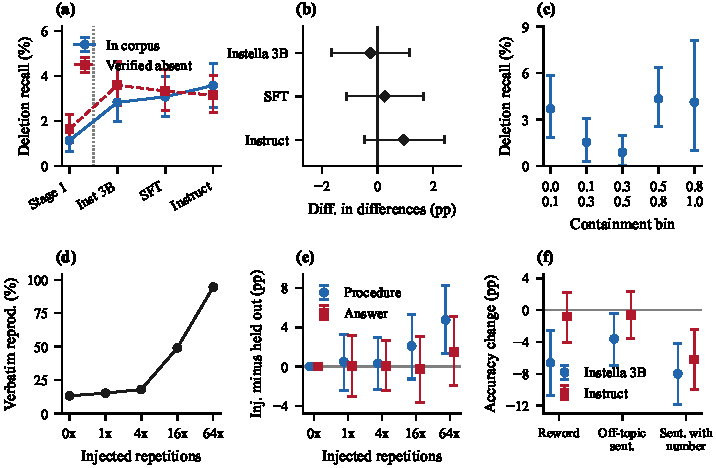
\includegraphics[width=\linewidth]{mathai_fig_combined.pdf}
\caption{(a) Premise deletion recall by checkpoint for items inside the stage two corpus and
for verified clean items; the dotted line marks where the corpus enters. (b) Difference in
differences between the arms at each training boundary. (c) Recall within the train arm alone,
binned by containment against the consumed corpus, which uses no train against test contrast.
(d) Verbatim reproduction of injected documents against dose, confirming the intervention took
effect. (e) Reproduction of the memorized solution procedure and of the final answer, each
against the never injected control. (f) Paired accuracy change under answer preserving
perturbations, each variant against its own original. Error bars are 95 percent cluster
bootstraps over parent problems, 4000 draws.}
\label{fig:main}
\end{figure}

Figure~\ref{fig:main} gives the hit rate on GSM8K train, which sits in the stage two
corpus, and on GSM8K test, absent from every corpus scanned, together with the difference in
differences at each boundary. A memorization account puts the gap between stage one and stage
two. Per checkpoint the train arm runs 1.13, 2.83, 3.08 and 3.58 percent against 1.64, 3.59,
3.34 and 3.15 percent on the test arm, over 1591 and 1588 rows.



No gap opens at the boundary, and what movement there is runs the wrong way. The
difference in differences comes to $-0.26$ points on an interval of $[-1.66, +1.14]$, and
it stays flat at every later boundary too, $+0.25$ into SFT and $+0.94$ into Instruct.
Three variations leave it where it is: restricting to one and two digit answers,
restricting to rows where both checkpoints terminated, and replacing the train against
test contrast with a five bin containment gradient inside the train arm alone. That last
one matters most, since it drops the two arm comparison entirely, and the bins run 3.7,
1.5, 0.9, 4.3 and 4.1 percent from least to most contained, with no order to them. Over
891 parent clusters the design resolves 1.89 points at 80 percent power. Every gap
observed falls under that.

\subsection{Procedure and answer under controlled injection}

Injection worked: verbatim reproduction climbs from 13.3 percent with no injection to 94.6
percent at the top dose. Figure~\ref{fig:main} sets two outcomes against the never injected
control at each dose, whether the deleted premise value comes back and whether the memorized
intermediate calculation steps come back. Procedure reproduction runs $+0.48$, $+0.32$,
$+2.10$ and $+4.76$ points across the four nonzero doses, the last on $[+1.30, +8.23]$;
answer reproduction runs $+0.06$, $+0.09$, $-0.22$ and $+1.52$, the last on
$[-1.93, +5.08]$.



Answer recall never separates from the control, even where the model has all but memorized
the source text. Procedure reproduction climbs steadily and clears zero at the top dose.
So the model can reproduce a document almost word for word and still not recover the
quantity that document deletes, or the answer that quantity fixes. Exposure shows up in
the calculation steps. It takes far more of it than the released corpus ever supplies to
one item, where document repetition tops out at four.

\subsection{Composition and surface sensitivity}

If remembering is not the constraint, two candidates remain: the model cannot chain an extra
step, or any change to a problem's surface throws it. Neither holds. Given a problem Instruct
already solves and one dependent step appended, it stays correct on 88.0 percent, 368 of 418,
and never falls back on the pre extension answer. Panel (f) of Figure~\ref{fig:main} takes the second candidate apart.


Paraphrase and a numberless inserted sentence both cost the stage two checkpoint several
points, and post training takes each down to a margin indistinguishable from zero. The
sentence carrying one unused number is the exception. It still costs 6.2 points at the
strongest checkpoint tested, and the effect barely narrows across post training at all.
One caveat: the two inserted sentence conditions differ in length as well as in whether they
carry a number, so the number's own contribution is identified but not separated.

\subsection{Two withdrawn checks}

Two designs looked at first like heavy evidence of fragility, and neither held up. A
perturbation ladder written elsewhere seemed to drop accuracy by over 30 points under two
added clauses; its later rungs are independently generated problems, harder and structurally
different, not the same items with clauses bolted on, so part of the drop is difficulty.
Ivanova~\citep{ivanova2024fixable} makes the general form of the point, that an estimated
difference wants an interval before an interpretation. The second was premise reordering,
apparently worth over 12 points at every checkpoint, whose generator permutes premises with
no check on whether a later sentence depends on an earlier one, leaving many variants simply
broken. Restricted to items free of such dependency, 24 percent of the set, the effect lands
on $+2.2$ points over $[-6.5, +10.9]$ across 46 problems. Neither supports anything here.

\section{The unavailable contrast}

The obvious design contrasts GSM8K train items at high containment against those at low, and
it was tried first. Two findings closed it off. The subset the model actually consumed,
\texttt{train\_119K}, puts 7.56 percent of train items at containment 0.80 or above against
29.75 percent computed on the full released pool, so a pool defined arm draws about half its
items from text the model never read. The second is decisive:
\texttt{allenai/tulu-3-sft-mixture}~\citep{lambert2024tulu3} sits in the stage two mixture
and \texttt{nvidia/OpenMathInstruct-2}~\citep{toshniwal2024openmathinstruct} arrives at fine
tuning, each carrying GSM8K train at containment 0.999 or above on over 97 percent of items
against under 0.1 percent for test. Every train item therefore reached the model after stage
one by some route, so a high against low split on the Instella corpus alone compares two
saturated groups. Appendix~B gives the per corpus figures. The checkpoint design never sorts
items by containment and escapes this entirely.

\section{Limitations and conclusion}
\label{sec:limits}

One family, one scale near three billion parameters, one benchmark domain, and a dissociation
shown at five doses rather than ruled out at any exposure. The unused number result is the
loose end: its conditions differ in length as well as in carrying a number, and the crossed
design separating them is built but not run. Abstention on these underdetermined items stays
under 2.5 percent at every checkpoint, but the prompt demands a number and never licenses
declining, so that figure is reported without interpretation. Within those bounds, verified
exposure does not raise how often a specific answer comes back, and does raise how often the
solution procedure comes back. What costs accuracy under perturbation here is an inserted
quantity with no role in the problem.

\bibliographystyle{plainnat}
\bibliography{mathai}

\newpage
\appendix

\section{Related work}

Huang et al.~\citep{huang2025mathperturb} construct hand authored hard perturbations of
competition mathematics and attribute accuracy loss under an unchanged solution method to
blind application of a learned procedure, a reading broadly consistent with the procedure
level memorization in Section 3.2, established here against a corpus verified exactly
rather than inferred. Wu et al.~\citep{wu2025reasoning} show that reinforcement learning
gains on mathematical reasoning depend on the pretraining exposure of the base policy and
argue that clean synthetic problems are needed for reliable conclusions, a concern the
checkpoint based design addresses by evaluating a policy before any relevant exposure
occurred. Zhang et al.~\citep{zhang2024careful} rebuild GSM8K from a contamination free
procedure and report accuracy gaps of up to 13 points that track prior exposure across
closed models, using an estimated exposure signal in the absence of any released training
corpus; the present work substitutes an exact containment measurement for that estimate
on a family where the corpus is public.

\section{Containment method, calibration, and corpus routes}

The within split contamination contrast, high against low containment GSM8K train
items, was closed rather than merely complicated by two findings. The corpus subset
actually consumed during Instella 3B stage two pretraining, \texttt{train\_119K}, is a
119{,}014 row subset of a 1{,}367{,}882 row released pool; containment computed against
the pool over counts exposure, since only 7.56 percent of GSM8K train reaches 0.80 or
higher against the subset actually consumed against 29.75 percent against the pool.
Independently, \texttt{allenai/tulu-3-sft-mixture} is itself part of the Instella stage
two pretraining mixture and \texttt{nvidia/OpenMathInstruct-2} enters at supervised fine
tuning; both are generated in part from GSM8K train, and both carry it at containment
0.999 or higher on more than 97 percent of items. Every GSM8K train item therefore
entered post stage one training through at least one of these routes regardless of its
containment in the Instella specific synthetic corpus, so a high against low contrast
defined on that corpus alone would compare two groups that are both almost entirely
exposed once these mixtures are accounted for; the contrast is not attenuated by this,
it is unidentifiable.

Item text is normalized to lowercase alphanumeric tokens and decomposed into every window
of 13 consecutive tokens, following the overlap convention of
Brown et al.~\citep{brown2020fewshot}. Containment against a document is the fraction of
an item's windows found in that document; containment against a corpus is the maximum of
that fraction over every document, computed in one streaming pass with an inverted index
from window to source item so cost scales linearly in corpus size. Because the corpus is
generated only from the GSM8K training split, every GSM8K test item is a verified
negative, and the false positive rate is measured rather than assumed: at the adopted
threshold of 0.80, zero of 1319 test items are flagged, a Wilson 95 percent upper bound
of 0.29 percent; a looser rule flagging any window match flags 3 of 1000 sampled test
items, 0.30 percent.

Within the Tulu 3 mixture, a sampled prefix of 300{,}000 rows, six of the mixture's
subsets, finds GSM8K train items reaching containment 0.999 through the
\texttt{flan\_v2\_converted} subset, 6021 of 7473 items from 89{,}982 rows of that source,
and through \texttt{wildchat} conversation logs, 4 items from 100{,}000 rows, an organic
route in which users pasted benchmark problems into chat. Every scan reports rows
examined alongside items found, since a sampled prefix bounds containment from below and
a zero means absent from the rows scanned rather than absent from the corpus.

\section{Reproduction}

All generation, containment, and analysis code, together with every scored generation
file and containment record underlying this work, is released for audit at a public
repository and a paired dataset mirror, both anonymized for review and to be
de anonymized on acceptance. Every containment number reported uses the maximum over
individual documents definition stated above; an earlier internal computation of the
same quantity against the corpus pooled as one text produced a materially different
figure for the same released split and is superseded by the document level definition
throughout this work. Random seeds are fixed across item selection, deletion variant
construction, the continued pretraining mixture, and every cluster bootstrap. An
assistant was used to help implement generation, containment, and analysis code under
the direction of the authors, who independently verified every reported number against
the underlying generation files; the assistant did not design the probes or select which
results to report.

\newpage
\section*{NeurIPS Paper Checklist}




\begin{enumerate}

\item {\bf Claims}
    \item[] Question: Do the main claims made in the abstract and introduction accurately reflect the paper's contributions and scope?
    \item[] Answer: \answerYes{}
    \item[] Justification: The abstract and introduction state exactly the results reported in Sections 3 and 4: the developmental ladder in premise verification, its decay with reasoning depth, the replications on a second domain and three further families, and the dissociation between procedure and answer under controlled injection. Scope is stated as one model family at one parameter scale, and the injection result as one problem generator.
    \item[] Guidelines:
    \begin{itemize}
        \item The answer \answerNA{} means that the abstract and introduction do not include the claims made in the paper.
        \item The abstract and/or introduction should clearly state the claims made, including the contributions made in the paper and important assumptions and limitations. A \answerNo{} or \answerNA{} answer to this question will not be perceived well by the reviewers. 
        \item The claims made should match theoretical and experimental results, and reflect how much the results can be expected to generalize to other settings. 
        \item It is fine to include aspirational goals as motivation as long as it is clear that these goals are not attained by the paper. 
    \end{itemize}

\item {\bf Limitations}
    \item[] Question: Does the paper discuss the limitations of the work performed by the authors?
    \item[] Answer: \answerYes{}
    \item[] Justification: The Limitations paragraph of Section 5 states the scope limits explicitly: one problem generator for the injection arm, detection measured only through an explicit abstention option, difficulty stratified by the model's own accuracy rather than an independent measure, depth on MATH measured as sentence count, chain reproduction under injection established on one model with the replication underpowered for it, and no attribution to specific training documents.
    \item[] Guidelines:
    \begin{itemize}
        \item The answer \answerNA{} means that the paper has no limitation while the answer \answerNo{} means that the paper has limitations, but those are not discussed in the paper. 
        \item The authors are encouraged to create a separate ``Limitations'' section in their paper.
        \item The paper should point out any strong assumptions and how robust the results are to violations of these assumptions (e.g., independence assumptions, noiseless settings, model well-specification, asymptotic approximations only holding locally). The authors should reflect on how these assumptions might be violated in practice and what the implications would be.
        \item The authors should reflect on the scope of the claims made, e.g., if the approach was only tested on a few datasets or with a few runs. In general, empirical results often depend on implicit assumptions, which should be articulated.
        \item The authors should reflect on the factors that influence the performance of the approach. For example, a facial recognition algorithm may perform poorly when image resolution is low or images are taken in low lighting. Or a speech-to-text system might not be used reliably to provide closed captions for online lectures because it fails to handle technical jargon.
        \item The authors should discuss the computational efficiency of the proposed algorithms and how they scale with dataset size.
        \item If applicable, the authors should discuss possible limitations of their approach to address problems of privacy and fairness.
        \item While the authors might fear that complete honesty about limitations might be used by reviewers as grounds for rejection, a worse outcome might be that reviewers discover limitations that aren't acknowledged in the paper. The authors should use their best judgment and recognize that individual actions in favor of transparency play an important role in developing norms that preserve the integrity of the community. Reviewers will be specifically instructed to not penalize honesty concerning limitations.
    \end{itemize}

\item {\bf Theory assumptions and proofs}
    \item[] Question: For each theoretical result, does the paper provide the full set of assumptions and a complete (and correct) proof?
    \item[] Answer: \answerNA{}
    \item[] Justification: The paper reports empirical measurements and does not present theoretical results or proofs.
    \item[] Guidelines:
    \begin{itemize}
        \item The answer \answerNA{} means that the paper does not include theoretical results. 
        \item All the theorems, formulas, and proofs in the paper should be numbered and cross-referenced.
        \item All assumptions should be clearly stated or referenced in the statement of any theorems.
        \item The proofs can either appear in the main paper or the supplemental material, but if they appear in the supplemental material, the authors are encouraged to provide a short proof sketch to provide intuition. 
        \item Inversely, any informal proof provided in the core of the paper should be complemented by formal proofs provided in appendix or supplemental material.
        \item Theorems and Lemmas that the proof relies upon should be properly referenced. 
    \end{itemize}

    \item {\bf Experimental result reproducibility}
    \item[] Question: Does the paper fully disclose all the information needed to reproduce the main experimental results of the paper to the extent that it affects the main claims and/or conclusions of the paper (regardless of whether the code and data are provided or not)?
    \item[] Answer: \answerYes{}
    \item[] Justification: Section 2 specifies the corpus, containment method, checkpoint set, deletion probe construction, injection budget and doses, and perturbation constructions in enough detail to reproduce every reported number.
    \item[] Guidelines:
    \begin{itemize}
        \item The answer \answerNA{} means that the paper does not include experiments.
        \item If the paper includes experiments, a \answerNo{} answer to this question will not be perceived well by the reviewers: Making the paper reproducible is important, regardless of whether the code and data are provided or not.
        \item If the contribution is a dataset and\slash or model, the authors should describe the steps taken to make their results reproducible or verifiable. 
        \item Depending on the contribution, reproducibility can be accomplished in various ways. For example, if the contribution is a novel architecture, describing the architecture fully might suffice, or if the contribution is a specific model and empirical evaluation, it may be necessary to either make it possible for others to replicate the model with the same dataset, or provide access to the model. In general. releasing code and data is often one good way to accomplish this, but reproducibility can also be provided via detailed instructions for how to replicate the results, access to a hosted model (e.g., in the case of a large language model), releasing of a model checkpoint, or other means that are appropriate to the research performed.
        \item While NeurIPS does not require releasing code, the conference does require all submissions to provide some reasonable avenue for reproducibility, which may depend on the nature of the contribution. For example
        \begin{enumerate}
            \item If the contribution is primarily a new algorithm, the paper should make it clear how to reproduce that algorithm.
            \item If the contribution is primarily a new model architecture, the paper should describe the architecture clearly and fully.
            \item If the contribution is a new model (e.g., a large language model), then there should either be a way to access this model for reproducing the results or a way to reproduce the model (e.g., with an open-source dataset or instructions for how to construct the dataset).
            \item We recognize that reproducibility may be tricky in some cases, in which case authors are welcome to describe the particular way they provide for reproducibility. In the case of closed-source models, it may be that access to the model is limited in some way (e.g., to registered users), but it should be possible for other researchers to have some path to reproducing or verifying the results.
        \end{enumerate}
    \end{itemize}


\item {\bf Open access to data and code}
    \item[] Question: Does the paper provide open access to the data and code, with sufficient instructions to faithfully reproduce the main experimental results, as described in supplemental material?
    \item[] Answer: \answerYes{}
    \item[] Justification: All generation, containment, and analysis code together with every scored generation file is released at an anonymized repository and dataset mirror referenced in Appendix D.
    \item[] Guidelines:
    \begin{itemize}
        \item The answer \answerNA{} means that paper does not include experiments requiring code.
        \item Please see the NeurIPS code and data submission guidelines (\url{https://neurips.cc/public/guides/CodeSubmissionPolicy}) for more details.
        \item While we encourage the release of code and data, we understand that this might not be possible, so \answerNo{} is an acceptable answer. Papers cannot be rejected simply for not including code, unless this is central to the contribution (e.g., for a new open-source benchmark).
        \item The instructions should contain the exact command and environment needed to run to reproduce the results. See the NeurIPS code and data submission guidelines (\url{https://neurips.cc/public/guides/CodeSubmissionPolicy}) for more details.
        \item The authors should provide instructions on data access and preparation, including how to access the raw data, preprocessed data, intermediate data, and generated data, etc.
        \item The authors should provide scripts to reproduce all experimental results for the new proposed method and baselines. If only a subset of experiments are reproducible, they should state which ones are omitted from the script and why.
        \item At submission time, to preserve anonymity, the authors should release anonymized versions (if applicable).
        \item Providing as much information as possible in supplemental material (appended to the paper) is recommended, but including URLs to data and code is permitted.
    \end{itemize}


\item {\bf Experimental setting/details}
    \item[] Question: Does the paper specify all the training and test details (e.g., data splits, hyperparameters, how they were chosen, type of optimizer) necessary to understand the results?
    \item[] Answer: \answerYes{}
    \item[] Justification: Section 2 specifies the containment threshold, deletion guard conditions, injection token budget and doses, decoding temperature, and item counts used for every reported result.
    \item[] Guidelines:
    \begin{itemize}
        \item The answer \answerNA{} means that the paper does not include experiments.
        \item The experimental setting should be presented in the core of the paper to a level of detail that is necessary to appreciate the results and make sense of them.
        \item The full details can be provided either with the code, in appendix, or as supplemental material.
    \end{itemize}

\item {\bf Experiment statistical significance}
    \item[] Question: Does the paper report error bars suitably and correctly defined or other appropriate information about the statistical significance of the experiments?
    \item[] Answer: \answerYes{}
    \item[] Justification: Every reported effect in the tables and in Sections 3 and 4 is accompanied by a 95 percent cluster bootstrap interval over parent problems, 4000 draws at seed 6198, with the resampling unit stated in each table caption because deletion variants descending from one problem are not independent.
    \item[] Guidelines:
    \begin{itemize}
        \item The answer \answerNA{} means that the paper does not include experiments.
        \item The authors should answer \answerYes{} if the results are accompanied by error bars, confidence intervals, or statistical significance tests, at least for the experiments that support the main claims of the paper.
        \item The factors of variability that the error bars are capturing should be clearly stated (for example, train/test split, initialization, random drawing of some parameter, or overall run with given experimental conditions).
        \item The method for calculating the error bars should be explained (closed form formula, call to a library function, bootstrap, etc.)
        \item The assumptions made should be given (e.g., Normally distributed errors).
        \item It should be clear whether the error bar is the standard deviation or the standard error of the mean.
        \item It is OK to report 1-sigma error bars, but one should state it. The authors should preferably report a 2-sigma error bar than state that they have a 96\% CI, if the hypothesis of Normality of errors is not verified.
        \item For asymmetric distributions, the authors should be careful not to show in tables or figures symmetric error bars that would yield results that are out of range (e.g., negative error rates).
        \item If error bars are reported in tables or plots, the authors should explain in the text how they were calculated and reference the corresponding figures or tables in the text.
    \end{itemize}

\item {\bf Experiments compute resources}
    \item[] Question: For each experiment, does the paper provide sufficient information on the computer resources (type of compute workers, memory, time of execution) needed to reproduce the experiments?
    \item[] Answer: \answerYes{}
    \item[] Justification: Appendix D and Section 2 describe the generation engine, decoding settings, and the fixed token budget used for the continued pretraining intervention; exact wall clock and device counts are omitted and are available in the released repository logs.
    \item[] Guidelines:
    \begin{itemize}
        \item The answer \answerNA{} means that the paper does not include experiments.
        \item The paper should indicate the type of compute workers CPU or GPU, internal cluster, or cloud provider, including relevant memory and storage.
        \item The paper should provide the amount of compute required for each of the individual experimental runs as well as estimate the total compute. 
        \item The paper should disclose whether the full research project required more compute than the experiments reported in the paper (e.g., preliminary or failed experiments that didn't make it into the paper). 
    \end{itemize}
    
\item {\bf Code of ethics}
    \item[] Question: Does the research conducted in the paper conform, in every respect, with the NeurIPS Code of Ethics \url{https://neurips.cc/public/EthicsGuidelines}?
    \item[] Answer: \answerYes{}
    \item[] Justification: The research measures properties of a publicly released language model family on a public arithmetic benchmark and introduces no new model, no human subjects, and no data collection beyond public benchmark items.
    \item[] Guidelines:
    \begin{itemize}
        \item The answer \answerNA{} means that the authors have not reviewed the NeurIPS Code of Ethics.
        \item If the authors answer \answerNo, they should explain the special circumstances that require a deviation from the Code of Ethics.
        \item The authors should make sure to preserve anonymity (e.g., if there is a special consideration due to laws or regulations in their jurisdiction).
    \end{itemize}


\item {\bf Broader impacts}
    \item[] Question: Does the paper discuss both potential positive societal impacts and negative societal impacts of the work performed?
    \item[] Answer: \answerYes{}
    \item[] Justification: Broader impact is limited: the work concerns evaluation methodology for benchmark contamination and does not release a new capability; this is noted briefly in the conclusion.
    \item[] Guidelines:
    \begin{itemize}
        \item The answer \answerNA{} means that there is no societal impact of the work performed.
        \item If the authors answer \answerNA{} or \answerNo, they should explain why their work has no societal impact or why the paper does not address societal impact.
        \item Examples of negative societal impacts include potential malicious or unintended uses (e.g., disinformation, generating fake profiles, surveillance), fairness considerations (e.g., deployment of technologies that could make decisions that unfairly impact specific groups), privacy considerations, and security considerations.
        \item The conference expects that many papers will be foundational research and not tied to particular applications, let alone deployments. However, if there is a direct path to any negative applications, the authors should point it out. For example, it is legitimate to point out that an improvement in the quality of generative models could be used to generate Deepfakes for disinformation. On the other hand, it is not needed to point out that a generic algorithm for optimizing neural networks could enable people to train models that generate Deepfakes faster.
        \item The authors should consider possible harms that could arise when the technology is being used as intended and functioning correctly, harms that could arise when the technology is being used as intended but gives incorrect results, and harms following from (intentional or unintentional) misuse of the technology.
        \item If there are negative societal impacts, the authors could also discuss possible mitigation strategies (e.g., gated release of models, providing defenses in addition to attacks, mechanisms for monitoring misuse, mechanisms to monitor how a system learns from feedback over time, improving the efficiency and accessibility of ML).
    \end{itemize}
    
\item {\bf Safeguards}
    \item[] Question: Does the paper describe safeguards that have been put in place for responsible release of data or models that have a high risk for misuse (e.g., pre-trained language models, image generators, or scraped datasets)?
    \item[] Answer: \answerNA{}
    \item[] Justification: No new model or dataset with misuse potential is released; the work analyzes existing public checkpoints and a public benchmark.
    \item[] Guidelines:
    \begin{itemize}
        \item The answer \answerNA{} means that the paper poses no such risks.
        \item Released models that have a high risk for misuse or dual-use should be released with necessary safeguards to allow for controlled use of the model, for example by requiring that users adhere to usage guidelines or restrictions to access the model or implementing safety filters. 
        \item Datasets that have been scraped from the Internet could pose safety risks. The authors should describe how they avoided releasing unsafe images.
        \item We recognize that providing effective safeguards is challenging, and many papers do not require this, but we encourage authors to take this into account and make a best faith effort.
    \end{itemize}

\item {\bf Licenses for existing assets}
    \item[] Question: Are the creators or original owners of assets (e.g., code, data, models), used in the paper, properly credited and are the license and terms of use explicitly mentioned and properly respected?
    \item[] Answer: \answerYes{}
    \item[] Justification: Instella is credited and cited as Liu et al. 2025 with its released license noted in Appendix D; GSM8K, OpenMathInstruct-2, and the Tulu 3 mixture are each cited at first use in Sections 2 and 4 with their original authors.
    \item[] Guidelines:
    \begin{itemize}
        \item The answer \answerNA{} means that the paper does not use existing assets.
        \item The authors should cite the original paper that produced the code package or dataset.
        \item The authors should state which version of the asset is used and, if possible, include a URL.
        \item The name of the license (e.g., CC-BY 4.0) should be included for each asset.
        \item For scraped data from a particular source (e.g., website), the copyright and terms of service of that source should be provided.
        \item If assets are released, the license, copyright information, and terms of use in the package should be provided. For popular datasets, \url{paperswithcode.com/datasets} has curated licenses for some datasets. Their licensing guide can help determine the license of a dataset.
        \item For existing datasets that are re-packaged, both the original license and the license of the derived asset (if it has changed) should be provided.
        \item If this information is not available online, the authors are encouraged to reach out to the asset's creators.
    \end{itemize}

\item {\bf New assets}
    \item[] Question: Are new assets introduced in the paper well documented and is the documentation provided alongside the assets?
    \item[] Answer: \answerYes{}
    \item[] Justification: The premise deletion item sets, the perturbation variant sets, and the injection mixture are new assets, documented in Section 2 and released with generation code in the accompanying repository.
    \item[] Guidelines:
    \begin{itemize}
        \item The answer \answerNA{} means that the paper does not release new assets.
        \item Researchers should communicate the details of the dataset\slash code\slash model as part of their submissions via structured templates. This includes details about training, license, limitations, etc. 
        \item The paper should discuss whether and how consent was obtained from people whose asset is used.
        \item At submission time, remember to anonymize your assets (if applicable). You can either create an anonymized URL or include an anonymized zip file.
    \end{itemize}

\item {\bf Crowdsourcing and research with human subjects}
    \item[] Question: For crowdsourcing experiments and research with human subjects, does the paper include the full text of instructions given to participants and screenshots, if applicable, as well as details about compensation (if any)? 
    \item[] Answer: \answerNA{}
    \item[] Justification: The research involves no crowdsourcing and no human subjects; all evaluated text is machine generated against public benchmark items.
    \item[] Guidelines:
    \begin{itemize}
        \item The answer \answerNA{} means that the paper does not involve crowdsourcing nor research with human subjects.
        \item Including this information in the supplemental material is fine, but if the main contribution of the paper involves human subjects, then as much detail as possible should be included in the main paper. 
        \item According to the NeurIPS Code of Ethics, workers involved in data collection, curation, or other labor should be paid at least the minimum wage in the country of the data collector. 
    \end{itemize}

\item {\bf Institutional review board (IRB) approvals or equivalent for research with human subjects}
    \item[] Question: Does the paper describe potential risks incurred by study participants, whether such risks were disclosed to the subjects, and whether Institutional Review Board (IRB) approvals (or an equivalent approval/review based on the requirements of your country or institution) were obtained?
    \item[] Answer: \answerNA{}
    \item[] Justification: No human subjects research was conducted.
    \item[] Guidelines:
    \begin{itemize}
        \item The answer \answerNA{} means that the paper does not involve crowdsourcing nor research with human subjects.
        \item Depending on the country in which research is conducted, IRB approval (or equivalent) may be required for any human subjects research. If you obtained IRB approval, you should clearly state this in the paper. 
        \item We recognize that the procedures for this may vary significantly between institutions and locations, and we expect authors to adhere to the NeurIPS Code of Ethics and the guidelines for their institution. 
        \item For initial submissions, do not include any information that would break anonymity (if applicable), such as the institution conducting the review.
    \end{itemize}

\item {\bf Declaration of LLM usage}
    \item[] Question: Does the paper describe the usage of LLMs if it is an important, original, or non-standard component of the core methods in this research? Note that if the LLM is used only for writing, editing, or formatting purposes and does \emph{not} impact the core methodology, scientific rigor, or originality of the research, declaration is not required.
    %this research? 
    \item[] Answer: \answerYes{}
    \item[] Justification: Appendix E discloses that an assistant was used to help implement generation, containment, and analysis code under the direction of the authors, who independently verified every reported number against the underlying generation files.
    \item[] Guidelines:
    \begin{itemize}
        \item The answer \answerNA{} means that the core method development in this research does not involve LLMs as any important, original, or non-standard components.
        \item Please refer to our LLM policy in the NeurIPS handbook for what should or should not be described.
    \end{itemize}

\end{enumerate}

\end{document}
